\documentclass[../main.tex]{subfiles}
%\graphicspath{{\subfix{images/}}}


\begin{document}
\label{section:rlwe}

LWE's hardness proof using a combination of quantum and classical reductions sparked many LWE-based cryptosystems, which are deemed more practical in terms of the public key size and ciphertext expansion while maintaining the same provable security as those based on SIS. The quadratic key size in the security parameter $n$, however, is still a serious constraint for practical applications of LWE. In this section, we introduce an efficient variation of LWE, called \textbf{ring learning with errors} or ring-LWE (\textbf{RLWE}). The problem originated from LWE, but focused on ideal lattices that were discussed in the previous section, which are images of fractional ideals\index{fractional ideal} in a number field $K$ under the canonical embedding. As we will see, these lattices have additional algebraic properties that allows the public key size to be reduced to $\Tilde{O}(n)$ while retaining almost identical provable security.


\subsection{RLWE in cyclotomic field}

We first introduce the RLWE problem in the special case of a cyclotomic field, which is the most common setting for RLWE-based cryptosystems. 
A more general definition will be introduced in the next subsection.  

Recall the $m$th cyclotomic polynomial $\Phi_m(x)$ is the polynomial whose roots are the primitive $m$th roots of unity. As we have seen in Remark \ref{rmk:speCycPoly}, when $m=2n=2^k \ge 2$ is a positive power of 2, the cyclotomic polynomial has the simple form $\Phi_m(x)=x^n+1$. 
Let $R=\Z[x]/(\Phi_m(x))$ be a ring of integer coefficient polynomials modulo the cyclotomic polynomial. This is the primary domain where RLWE is defined in the special case. 
There are two interpretations of $R$. 
\begin{enumerate}\itemsep1mm\parskip0mm
    \item $R = \Z[x]/(x^n+1)$ is a quotient ring where every polynomial in $R$ has integer coefficients and degree less than $n$.
    \item $R = \Z[x]/(\Phi_m(x))$ is isomorphic to $\Z[\zeta_m]$, the ring of integers $\ok$ for the $m$-th cyclotomic field $K=\Q(\zeta_m)$. (See Theorem~\ref{thm:ring LWE isomoprhic 2}; Lemma~\ref{lm:difIdeal} motivates the specific choice of $m$.)
    % Second, let $K=\Q(\zeta_m)$ be the $m$th cyclotomic field, then $R=\ok$ is the ring of integers obtained by adjoining $\zeta_m$ to $\Z$, i.e., $R=\Z[\zeta_m]$.
\end{enumerate} 
 The first interpretation is the natural interpretation but the second interpretation is more useful when proving hardness result of RLWE. We have been through some important properties of $\ok$ such as its fractional ideals form a UFD and its geometric interpretation under the canonical embedding. 

Similar to the LWE, where elements are sampled from a finite field by taking $\Z_q = \Z \bmod q$ for a prime $q$, RLWE is also formulated in a finite field by taking $R$ modulo a prime $q$. This gives a domain $R_q=\Z_q[x]/(\Phi_m(x))$, which is a field of order $q^n$ by Theorem \ref{thm:quoRngIsField} because $\Phi_m(x)$ is monic irreducible. The field $R_q$ is the underlying domain for generating random RLWE elements. From here, we can define the RLWE distribution as follows. 

\begin{definition}
\label{def:rlwe1}
Given the following parameters
\begin{itemize}\itemsep1mm\parskip0mm
    \item $n$ - the security parameter that satisfies $n=2^k$ for an integer $k \ge 0$,
    \item $q$ - a large (public) prime modulus that is polynomial in $n$ and satisfies $q \equiv 1 \bmod 2n$,
\end{itemize}
for a fixed $\vc{s} \in R_q$ and an error distribution $\chi$ over $R$ that is concentrated on ``small integer'' coefficients, the \textbf{RLWE distribution} 
\reversemarginpar
\marginnote{\textit{RLWE distribution}}
over $R_q \times R_q$, denoted by 
\begin{equation*}
    RLWE(n,q,\chi) := \{(\vc{a},\vc{b})\}
\end{equation*}
is obtained by repeating these steps 
\begin{itemize}\itemsep1mm\parskip0mm
    \item sample an element $\vc{a} \leftarrow R_q$,
    \item sample a noise element $\vc{\epsilon} \leftarrow \chi$ over $R$,
    \item compute the polynomial $\vc{b} = \vc{s} \star \vc{a} + \vc{\epsilon} \bmod R_q$,
    \item output $(\vc{a},\vc{b})$.
\end{itemize}
\end{definition}

We use $\vc{f} \star \vc{g}$ to denote polynomial multiplication in order to distinguish it from vector dot product. From Section~\ref{subsec:canonical embedding}, we know that polynomial addition and multiplication can be done efficiently under the canonical embedding. 
The $\bmod \,R_q$ operation is as defined in Equation~(\ref{eq:modulo lattice}).

The RLWE problem also has a search version and a decision version. Just like in LWE, the former tries to solve for the secret polynomial $\vc{s}$ from RLWE samples whilst the latter tries to distinguish RLWE samples from uniformly random samples over the same domain. The reduction from search to decision RLWE, however, is not as simple as that in LWE. We will sketch the reduction in a later subsection. 

%An alternative way of interpreting the quotient ring $R$ is to view it as the ring of integers in a number field. We know the field of rationals adjoining with an $m$th primitive root of unity $\zeta_m$ gives a cyclotomic number field $K=\Q(\zeta_m)$ and its ring of integers is $\ok=\Z[\zeta_m]$. By Theorem \ref{thm:fieldExtEquiv}, the cyclotomic field is equivalent to $\Q(\zeta_m) \cong \Q[x] / (\Phi_m(x))$ and hence we have $\Z[\zeta_m] \cong \Z[x] / (\Phi_m(x))$. Therefore, the quotient ring $R=\Z[\zeta_m]$ is just the ring of integers in the $m$th cyclotomic field $K=\Q(\zeta_m)$. The reason to think $R$ this way is to build the connection with ideal lattices using existing algebraic tools that we have learned. From the previous section we know that ideal lattices are images of ideals or more generally fractional ideals of the ring of integers $R$ under the canonical embedding. With this connection, we can then prove that several ideal lattice problems reduce to the search RLWE problem. 

\iffalse
Both the coefficient and CRT representations can express a polynomial in a vector format. The reduction of the RLWE public key size is because of the reuse of the same polynomial $\vc{a}$, but with its vector components rotated and negated one at a time. This rotation and negation process is sometimes called \textit{anti-cyclic}. It allows each randomly sampled degree $n$ polynomial to be reused $n-1$ times and hence saves the storage for the public key. 
By definition, each polynomial $\vc{a}$ must be a sample of $R_q$. This is fine with the anti-cyclic action, because
each round of rotation and negation is equivalent to multiplying $\vc{a}$ by the polynomial $\vc{x} \in R$, which outputs a ``new'' polynomial that is still in the ring $R$. For example, let $R=\Z[x]/(x^4+1)$, given a polynomial $\vc{a} = 1+2x+3x^2+4x^3 \in R$ that is also expressed as $\vc{a}=(1,2,3,4)$ as shown by the top left array in Figure \ref{fig:antiCyc}. The anti-cyclic action is equivalent to $\vc{a} \star \vc{x} = x+2x^2+3x^3+4x^4=-4+x+2x^2+3x^3$. Multiplying $\vc{a}$ by $\vc{x}$ four times, we obtain $-\vc{a}$ which is almost identical to $\vc{a}$, so the polynomial can be reused for at most 3 times. 

\begin{figure}[ht]
    \centering
    \includegraphics[page=9]{images/Lattice_crypto_tikz_folder.pdf}
    \caption{Let $R=\Z[x]/(x^4+1)$. Given the polynomial $\vc{a}=1+2x+3x^2+4x^3$, the anti-cyclic action is equivalent to multiplying $\vc{a}$ by $\vc{x}$. After $n=4$ rounds of anti-cyclic actions, we get back to $-\vc{a}$, so each randomly sampled polynomial is reused $n-1$ times before sampling the next one. This greatly reduced the public key size in RLWE-based cryptosystems.}
    \label{fig:antiCyc}
\end{figure}
\fi

% The reuse of the same polynomial greatly reduced the public key size of RLWE-based cryptosystems. 
In a LWE-based cryptosystems, as shown in Section \ref{subsec:lweSecurity}, the public key is $(\vc{A},\vc{b})$ where $\vc{A} \in \Z_q^{n \times m}$ is a matrix that needs $O(mn)$ storage. 
For an RLWE-based cryptosystem, the public key size can be reduced to $O(n)$, which is a significant saving in terms of storage. 
The reason is because each sample from an RLWE distribution is a pair of $n$-degree polynomials (Definition~\ref{def:rlwe2}) that can replace $n$ samples from the standard LWE distribution (Definition~\ref{def:lweDist}).

\iffalse
There are two questions that we would like to investigate in this section. First, given the public key is not completely random in RLWE-based cryptosystems, do we still get the same level of protection as in LWE? Second, why does this not work in general lattices like in LWE? More specifically, if we also reuse each random vector $\vc{a} \in \Z_q^n$ in LWE, can it still provide the same level of protection as before? 
\fi

\subsection{RLWE in general number field}

% To generalize the concept of RLWE to a broader context, we need to introduce a few more definitions and notations.

\iffalse
%We first introduce the basics of tensor product, which will be used through out RLWE representations and proofs. 
Given two $R$-modules $M$ and $N$, we can define a map $f:M \times N \rightarrow Q$. The map is called \textbf{$R$-bilinear} if it is linear at each component. More precisely, for all $m, m' \in M$ and $n, n' \in N$ and $r \in R$, the map $f$ is an $R$-bilinear map if the following are satisfied: 
\begin{align*}
    f(m+m',n) &= f(m,n)+f(m',n) \\
    f(m,n+n') &= f(m,n)+f(m,n')\\
    f(rm,n)&=rf(m,n)=f(m,rn).
\end{align*}
The image $Q$ of $f$ is also an $R$-module and together with the function $f$, they make the tensor product of $M$ and $N$. 

% see JS Milne, page 21
\begin{definition}
Given two $R$-modules $M$ and $N$ and an $R$-bilinear map $f: M\times N \rightarrow Q$, the pair $(Q,f)$ is the \textbf{tensor product} of $M$ and $N$, denoted by $M \otimes_R N$, if every other $R$-bilinear map $g:M\times N \rightarrow P$ is a unique composition $g=\alpha \circ f$ of $f$ and an $R$-linear map $\alpha: Q\rightarrow P$.
\end{definition}
\fi 

In the generalized RLWE distribution definition, \cite{lyubashevsky2010ideal} used the notation $K_{\C} = K \otimes_{\Q} \C$ to denote the tensor product\index{tensor product} between the number field $K$ and $\C$, both of which are $\Q$-modules. % \footnote{In fact, the authors used $K_{\R} = K \otimes_{\Q} \R$. But I think $K_{\C}$ is a better one to use.} 
This tensor product $K_{\C}$, which essentially is an $\Q$-module is where the RLWE errors are sampled from according to a certain error distribution $\psi$. It is often convenient to think of $K_{\C}$ as the canonical space $H$, where an isomorphism exists between them. We will not prove the isomorphism, but just give an intuition. For an $n$-dimensional number field $K=\Q(\alpha)$ and the minimal polynomial $f(x) \in \Q[x]$ of the primitive element $\alpha$, the connection is built through the following isomorphisms 
\begin{align*}
    K \otimes_{\Q} \C \cong \left( \Q[x]/(f(x)) \right) \otimes_{\Q} \C \cong \C[x] / (f(x))
    % see JS Milne, page 23 for details of the first 2 isomorphisms
\end{align*}
and the fact that the minimal polynomial $f(x)=f_1(x) \cdots f_n(x)$ can be factored into linear factors in the complex space $\C$. So we have an isomorphism between $K_{\C}$ and the canonical space $H$ as 
\begin{align*}
    K_{\C} = K \otimes_{\Q} \C \cong \prod_{i=1}^n \C[x]/(f_i(x))=H.
\end{align*}

The RLWE errors are sampled from $K_{\C}$ and followed by modulo $\dual{R}$ to reduce them to within the dual lattice. For a number field $K$ and its ring of integers $R=\ok$, let $R_q=R/qR$ and $\dual{R}_q=\dual{R}/q\dual{R}$ and $\T = K_{\C} / \dual{R}$ (a high-dimensional torus). The following RLWE definition generalizes Definition \ref{def:rlwe1} to an arbitrary number field. 

\begin{definition}
\label{def:rlwe2}
Given the following parameters
\begin{itemize}\itemsep1mm\parskip0mm
    \item $n$ - the security parameter that satisfies $n=2^k$ for an integer $k \ge 0$,
    \item $q$ - a large (public) prime modulus that is polynomial in $n$ and satisfies $q \equiv 1 \bmod 2n$,
\end{itemize}
for a fixed $\vc{s} \in \dual{R}_q$ and an error distribution $\psi$ over $K_{\C}$, the \textbf{RLWE distribution} $A_{s,\psi}$ over $R_q \times \T$,
\reversemarginpar
\marginnote{\textit{RLWE distribution}}  
is obtained by repeating these steps
\begin{itemize}\itemsep1mm\parskip0mm
    \item sample an element $\vc{a} \leftarrow R_q$,
    \item sample a noise element $\vc{\epsilon} \leftarrow \psi$ over $K_{\C} \cong H$,
    \item compute the polynomial $\vc{b} = (\vc{s} \star \vc{a})/q + \vc{\epsilon} \bmod \dual{R}$,
    \item output $(\vc{a},\vc{b})$.
\end{itemize} 
\end{definition}

Here, we make some observations of this definition. First, as $R \subseteq \dual{R}$, the product $\vc{s} \star \vc{a} \in \dual{R}_q$ and $(\vc{s} \star \vc{a})/q \in \dual{R}$. The error $\vc{\epsilon}$ is taken from $K_{\C} \cong H$ but can be thought of as further reduced to within the dual $\dual{R}$ when computing $\vc{b}$ by $\bmod \dual{R}$. So the definition is in direct analogy of the LWE distribution. 

Second, the previous definition of RLWE in cyclotomic field is a special case of this. Although in this general setting, $\vc{a}$ and $\vc{s}$ are taken from $R_q$ and its dual $\dual{R}_q$ respectively, when $K$ is a cyclotomic field for $\Phi_m(x)$ where $m$ is a power of 2, it has been shown in Example~\ref{ex:dualL} that 
\reversemarginpar
\marginnote{\textit{$R=n\dual{R}$}}
\begin{equation}
\label{eq:scaleRDual}
    R=n\dual{R}.
\end{equation}
% at the end of Section \ref{subsec:dualLatInNumField}. 
Hence, it makes no difference that $\vc{s}$ and $\vc{a}$ are sampled from different domains in the cyclotomic field case. This relationship between $R$ and $\dual{R}$ is also used when reducing the search RLWE to decision RLWE later. 

Third, the error distribution $\psi$ above is not a 1-dimensional Gaussian distribution any more. Unlike in the LWE case where the 1-dimensional error $\epsilon$ is added to the dot product $\vc{a}\cdot \vc{s}$, in RLWE the $n$-dimensional error $\vc{\epsilon}$ is added to the resulting polynomial $\vc{a}\star \vc{s}$. Depending on how a polynomial is represented, the number of parameters in the high-dimensional error distribution varies. In the coefficient representation, the $n$-dimensional Gaussian error distribution is parameterized by the $n \times n$ covariance matrix. In contrast, in the canonical embedding representation, the same Gaussian distribution  $D_{\vc{r}}$ is the product of $n$ independent 1-dimensional Gaussian with either the same or different scales $\vc{r}=(r_1, \dots, r_n)$. (This is another justification for using canonical embedding in RLWE.) When $\vc{r}$ is a constant vector, $D_{\vc{r}}$ is called a \textbf{spherical Gaussian distribution}, otherwise it is called an \textbf{elliptical Gaussian distribution}. % \kl{They can be made equivalent.}

The issue of using a high-dimensional error distribution appears in the reduction from ideal lattice problems to RLWE. As discussed after the LWE hardness proof, the error can be adjusted relatively easily to meet the required error distribution of an LWE oracle in order to build a reduction from BDD. But in the RLWE case, there is no straightforward error adjustment to meet the target high-dimensional error distribution for the RLWE oracle, so the proof has to assume the RLWE oracle works for a wide range of error distributions that are defined next. 

\begin{definition}
For $\alpha > 0$, the set $\Psi_{\le \alpha}$ consists of all elliptical Gaussian distributions $D_{\vc{r}}$ over $K_{\C}$ such that each $D_{r_i}$ has scale $r_i \le \alpha$.
\end{definition}

With this family of error distributions, we can define the search RLWE problem as follows.

\begin{definition}
\reversemarginpar
\marginnote{\textit{Search RLWE}}
Given the parameter $q$ and the family of error distributions $\Psi_{\le \alpha}$, the \textbf{search RLWE} problem, denoted by \textbf{RLWE$_{q,\Psi_{\le \alpha}}$}, is to compute the secret key $\vc{s}$  given samples $\{(\vc{a}, \vc{b})\}$ from the RLWE distribution $A_{\vc{s},\psi}$ for an arbitrary $\vc{s} \in \dual{R}_q$ and $\psi \in \Psi_{\le \alpha}$.
\end{definition}

The decision RLWE is an average case problem for a random secret key and a random error distribution. The distribution for the secret key $\vc{s}$ is uniform over the dual lattice $\dual{R}$. The distribution $\Upsilon_{\alpha}$ over the elliptical Gaussian error distributions $\Psi_{\le \alpha}$ is defined based on a Gamma distribution with shape 2 and scale 1.\footnote{\cite{lyubashevsky2010ideal} emphasized that any efficiently samplable continuous distributions can be used, e.g., Gaussian distribution.} Since the reduction from search to decision RLWE can only be made possible in cyclotomic number fields, we define $\Upsilon_{\alpha}$ specifically within cyclotomic number fields. Recall that for $m=2n=2^k > 2$, the canonical embedding for a cyclotomic number field $K=\Q(\zeta_m)$ consists only $n$ complex embeddings which are in $n/2$ conjugate pairs $\sigma_i=\overline{\sigma_{i+n/2}}$ for $i \in [0,n/2]$, so the scale parameters correspond to each conjugate pair of complex embeddings are made identical. This gives rise to the next definition of the distribution $\Upsilon_{\alpha}$. 

\begin{definition}
For $m=2n=2^k > 2$ an integer power of 2, let $K=\Q(\zeta_m)=\Q[x]/(x^n+1)$ be the $m$th cyclotomic field. For a real $\alpha>0$, let $\Upsilon_{\alpha}$ be the \textbf{distribution over the family} $\Psi_{\le \alpha}$ of elliptical Gaussian distributions. Then every element $\psi$ sampled from $\Upsilon_{\alpha}$ is an elliptical Gaussian distribution $D_{\vc{r}}$ over $K_{\C}$ whose scale parameters $r_i^2 = r_{i+n/2}^2=\alpha^2(1+\sqrt{n} x_i)$, where $x_1, \dots, x_{n/2}$ are chosen independently from the Gamma distribution $\Gamma(2,1)$.
\end{definition}

Using this definition, we define the average-case decision version of RLWE as follows. 

\begin{definition}
\reversemarginpar
\marginnote{\textit{Decision RLWE}}
Given the parameter $q$ and a distribution $\Upsilon_{\alpha}$ over the family $\Psi_{\le \alpha}$ of elliptical Gaussian distributions, the \textbf{average-case decision RLWE} problem, denoted by RDLWE$_{q, \Upsilon_{\alpha}}$, is to distinguish between samples from the RLWE distribution $A_{\vc{s},\psi}$ for a random choice of $(\vc{s},\psi) \leftarrow U(\dual{R}) \times \Upsilon_{\alpha}$ and the uniform samples from $R_q \times \T$.
\end{definition}

The mean of $\Gamma(2,1)$ is 2, by the above definition of $\Upsilon_{\alpha}$ we have $||r_i|| \approx O(\alpha n^{1/4})$. Recall that in the proof of LWE hardness, we discussed the upper bound of the scale parameter $\alpha$ in the Gaussian error distribution $\Psi_{\alpha}$ in order for $\Psi_{\alpha}$ to be distinguishable from the uniform distribution once reduced by $\bmod \,\Z_p^n$. The same argument carries over to the RLWE problem too, that is, $\psi \bmod \dual{R}$ and the uniform distribution over $\T=K_{\C}/\dual{R}$ should be distinguishable, for otherwise the decision RLWE is undefined. The difference is in the $n$th successive minima $\lambda_n(R)$. When $K$ is a cyclotomic number field, it has a power basis $\{1, \zeta, \dots, \zeta^{n-1} \}$, which is also a basis of $R$. Under the canonical embedding, each element $\zeta^k$ in the power basis is mapped to an element $(\sigma_1(\zeta^k), \dots, \sigma_n(\zeta^k))$ in the canonical space, where each $\sigma_i$ maps $\zeta^k$ to a different element in the power basis with $||\sigma_i(\zeta^k)||=1$. Hence, the Euclidean norm of $\zeta^k$'s image under the canonical embedding is $\sqrt{n}$ and $\lambda_n(R)=\sqrt{n}$. This implies the $n$th successive minima $\lambda_n(\dual{R})=1/\sqrt{n}$ and hence the upper bound of $\alpha$ in RLWE is $\alpha \le O(\sqrt{\log n/n})$, which is smaller than $O(\sqrt{\log n})$  in LWE. 

We now state the main theorem of RLWE in the specific context of cyclotomic number field and leave the proof to the following subsections. For the following theorem, let $K=\Q(\zeta_m)=\Q[x]/(x^n+1)$ be the $m$th cyclotomic number field and $R=\ok=\Z[x]/(x^n+1)$ be its ring of integers. 

\begin{theorem}
\label{thm:svpToRLWE}
\reversemarginpar
\marginnote{\textit{SVP, SIVP to RDLWE}}
Let $\alpha \in (0, \sqrt{\log n/n})$ and $q=q(n) \ge 2$ such that $q \equiv 1 \bmod m$ and $\alpha q \ge \omega(\log n)$. There are polynomial time quantum reductions from $\Tilde{O}(\sqrt{n}/\alpha)$-SIVP (or SVP) on ideal lattices in $K$ to 
\begin{itemize}
    \item RDLWE$_{q, \Upsilon_{\alpha}}$ and
    \item RDLWE$_{q, D_{\xi}}$ given only $l$ samples, where $\xi=\alpha (nl / \log(nl))^{1/4}$ is the scale parameter for the spherical Gaussian error distribution.
\end{itemize}
\end{theorem}

The first reduction is to the decision RLWE with a random elliptical Gaussian error distribution, whilst the second reduction is to the decision RLWE with a fixed spherical Gaussian error distribution but given only a small number $l$ of samples. We will make clear the connection between these two problems in a following subsection. % \kl{mention the ellipitcal gaussian incurs a factor $n^{1/4}$.}

\subsection{Ideal lattice problems}

Before going on to prove the hardness of RLWE, we re-define lattice problems in terms of ideal lattices in a number field that will be used  in the following proofs. 

Recall that an $n$-dimensional number field $K$ is mapped to the canonical space $H \cong \R^n$ by the canonical embedding, which also maps a fractional ideal\index{fractional ideal} $I$ of $K$ to an ideal lattice in $H$. 
Given a fractional ideal $I \subseteq K$ with the denominator $d \in \ok$, the corresponding integral ideal is $dI \subseteq \ok$. Since the norm $N(d)=\prod_{i=1}^n \sigma_i(d)$ where $\sigma_i$ is a real or complex embedding in the canonical embedding, we have $N(d) \in \langle d \rangle$ is in the principal ideal, i.e., $N(d)=k  d$ for an element $k \in K$. This implies that $N(d) I =k(dI) \subseteq  \ok$ is a scaled integral ideal. 
Hence, in the rest of this subsection, we define the three lattice problems in terms of ideal lattices that correspond to either a fractional ideal or a scaled integral ideal in the number field. 

Also recall that the canonical embedding enables us to talk about geometric norms of number field elements. In particular, we define the $L_p$-norm of an element $x \in K$ as 
\begin{equation*}
    ||x||_p = ||\sigma(x)||_p = 
    \begin{cases}
     \left( \sum_{i \in [n]} |\sigma_i(x)|^p \right)^{1/p} & \text{ if $p < \infty$},  \\
    \max_{i \in [n]} |\sigma_i(x)| & \text{ if $p = \infty$}.
    \end{cases}
\end{equation*}
With geometric norm, it makes sense to compare the lengths of two elements in a number field. 

\begin{tcolorbox}
\noindent
\textbf{The $\gamma$-Shortest Vectors Problem in $K$ (K-SVP$_{\gamma}$)}\\
Let $K$ be an $n$-dimensional number field. Given a fractional ideal\index{fractional ideal} $I$ of $K$, find a non-zero element $x \in I$ such that $||x||_p \le \gamma(n) \cdot \lambda_1(I)$.
\end{tcolorbox}

\begin{tcolorbox}
\noindent
\textbf{The $\gamma$-Shortest Independent Vectors Problem in $K$ (K-SIVP$_{\gamma}$)}\\
Let $K$ be an $n$-dimensional number field. Given a fractional ideal $I$ of $K$, find $n$ linearly independent non-zero elements $x_i, \dots, x_n \in I$ such that $\max_{i \in [1,n]} ||x_i||_p \le \gamma(n) \cdot \lambda_n(I)$.
\end{tcolorbox}

\begin{tcolorbox}
\noindent
\textbf{The $\alpha$-Bounded Distance Decoding in $K$ (K-BDD$_{\alpha}$)}\\
Let $K$ be an $n$-dimensional number field. Given a fractional ideal $I$ of $K$ and an element $y =x+e \in K$, where $x \in I$ and $||e||_{\infty} \le \alpha \cdot \lambda_1(I)$, find the element $x \in I$.
\end{tcolorbox}

\begin{tcolorbox}
\noindent
\textbf{The $\gamma$-Discrete Gaussian Sampling in $K$ (K-DGS$_{\gamma}$)}\\
Let $K$ be an $n$-dimensional number field. Given a fractional ideal\index{fractional ideal} $I$ of $K$ and a number $s \ge \gamma=\gamma(I)$, produce samples from the discrete Gaussian distribution $D_{I, s}$ over the ideal lattice $I$ with the scale $s$.
\end{tcolorbox}



\subsection{Hardness of search RLWE}

%x^n+1 should be irreducible over the integers, it can be reducible over p, that doesn't matter. 

In contrast to the big (and small) O notation, the small omega notation is used to denote a non-asymptotically tight lower bound of the function. That is, $f(n) = \omega(g(n))$ if for all $k>0$ there exists $n_0$ such that for all $n > n_0$ it satisfies $|f(n)|>k|g(n)|$. Throughout the proof, $\omega(\sqrt{\log n})$ is used to denote a function that grows asymptotically faster than  $\sqrt{\log n}$. 

\begin{figure}[hbt!]
    \centering
    \includegraphics[page=17]{images/Lattice_crypto_tikz_folder.pdf}
    \caption{Caption}
    \label{fig:rlweReduction}
\end{figure}

Similar to the LWE hardness proof, the hardness of RLWE relies on reductions from hard ideal lattice problems K-SVP$_\gamma$ and K-SIVP$_\gamma$, through the intermediate K-DGS problem. We omit the reductions from the two ideal lattice problems to K-DGS, but only focus on the quantum reduction to RLWE as stated in the next theorem. Note the context of this reduction is for arbitrary number fields that are not necessarily cyclotomic. 

\begin{theorem}
\label{thm:rlweIter}
\reversemarginpar
\marginnote{\textit{K-DGS to RLWE}}
Let $\alpha=\alpha(n)>0$ and $q=q(n) \ge 2$ such that $\alpha q \ge 2 \omega(\sqrt{\log n})$. There is a PPT quantum reduction from K-DGS$_{\gamma}$ to RLWE$_{q,\Psi_{\le \alpha}}$, where 
\begin{equation}
\label{equ:gamma}
    \gamma = \max\{\eta_{\epsilon}(I) (\sqrt{2}/\alpha) \omega(\sqrt{\log n}), \sqrt{2n}/\lambda_1(\dual{I})\}.
\end{equation}
\end{theorem}

Given $\alpha < \sqrt{\log n / n}$ as stated in Theorem \ref{thm:svpToRLWE} and the smoothing parameter $\eta_{\epsilon}(I) > 1/ \lambda_1(\dual{I})$ by Claim 2.13 \cite{regev2009lattices}, it always satisfies that $\gamma =\eta_{\epsilon}(I) (\sqrt{2}/\alpha) \omega(\sqrt{\log n})$. 

Again, the intuition behind the theorem is to obtain discrete Gaussian samples from an ideal lattice $I$ in $K$ with scale $s$ as close to the lower bound $\gamma$ as possible. The feasibility of obtaining such a short sample can be proved using almost the same strategy as LWE, that is, by using a classical reduction to solve the K-BDD problem with an RLWE oracle and the given discrete Gaussian samples with scale $r$, then feed the K-BDD output to a quantum algorithm to generate discrete Gaussian samples with scale $r' < r/2$. The combination of the classical and quantum algorithms, which is known as the iterative step in LWE, is the key to K-DGS for a small scale, see Figure \ref{fig:rlweReduction}. The classical reduction is stated in the next lemma. 

%this is lemma 4.3 in lyubashevsky2010ideal
\begin{lemma}
\reversemarginpar
\marginnote{\textit{K-BDD to RLWE}}
Let $\alpha =\alpha(n)> 0$, $q =q(n) \ge 2$ be an integer with known factorization. Let $I$ be a fractional ideal of a number field $K$ and $r\ge \sqrt{2} q \eta_{\epsilon}(I)$ for some negligible $\epsilon=\epsilon(n)$. Given a discrete Gaussian oracle for $D_{I,r}$, there is a PPT reduction from K-BDD$_d$ in the dual lattice $\dual{I}$ where $d=\alpha q / (\sqrt{2}r)$ to RLWE$_{q,\Psi_{\le \alpha}}$.
\end{lemma}

To solve the K-BDD problem for an element in the ideal lattice $I$ of $K$, the same bit-by-bit strategy as in Lemma \ref{lm:lweCoeffModQ} can be used here too. That is, find a solution in the scaled ideal lattice $qI$ and then iteratively build a solution in $I$ from the least to the most significant bit in the base $q$. Since Lemma \ref{lm:lweCoeffModQ} was proved for general lattices, it also holds for ideal lattices. The K-BDD problem in a scaled ideal lattice $qI$ is called $q$-BDD. 

Before proving the lemma, we recall two important CRT lemmas that will be employed to produce RLWE samples for an oracle. Both lemmas were introduced and proved in Section \ref{subsection:number field}, but in a more general context. Here, we re-state them in a number field $K$ and ring of integers $\ok$. The first lemma serves as a technical step to prove the second. 

% see lemma 5.2.2 in stein2012algebraic
\begin{lemma}
\label{lm:coprimeIdeals2}
If $I$ and $J$ are non-zero integral ideals of $R=\ok$, then there exists an element $t \in I$ such that $(t)\inv{I} \subseteq R$ is an integral ideal coprime to $J$. 
\end{lemma}

% state the lemma according to lemma 2.15 lyubashevsky2010ideal, which is a special case of prop 5.2.4 in stein2012algebraic.
\begin{lemma}
\label{lm:clearIdeals2}
Let $I$ and $J$ be ideals in $R=\ok$ and $M$ be a fractional ideal in the number field $K$. Then there is an isomorphism 
\begin{align*}
    M/JM \cong IM/IJM.
\end{align*}
\end{lemma}

As special cases of this lemma, we could let $J=(q)$ and $M=R$ be the ring of integers or $M=\dual{I}$ be the dual ideal. Given the prime factors of the integer $q$, say $q=ab$ where $a,b \in \Z$ are primes, the principal ideal can be written as $(q)=(a)(b)$ the product of prime ideals in $\Z$. Using a prime ideal factorization technique (will be briefly discussed in the next subsection), we can find the prime factors of $(a)$ and $(b)$ in $R$ hence $(q)$. It then follows from Lemma \ref{lm:coprimeIdeals2} that there is an element $t \in I$ to construct a coprime ideal $(t)\inv{I}$ to $J=(q)$ (see proofs of these lemmas in Section \ref{subsection:number field}, also see the proof of lemma 5.2.2 in \cite{stein2012algebraic} to see why we need to know the prime factors of the ideal $J$). Then the map 
\begin{align*}
    \theta_t: K &\rightarrow K \\
    u &\mapsto ut
\end{align*}
induces isomorphisms 
\begin{align}
\label{eq:theta1}
    R/(q)R = R_q & \cong IR/I(q)R =I_q\\
    \label{eq:theta2}
    \dual{I}/(q)\dual{I}=\dual{I}_q &\cong I\dual{I}/I(q)\dual{I}=I \inv{I}\dual{R}/I(q)\inv{I}\dual{R} = \dual{R}/(q)\dual{R}=\dual{R}_q.
\end{align}
Both induced isomorphisms in Equation \ref{eq:theta1} and \ref{eq:theta2} will be directly used in the hardness proof of q-BDD. We now state and prove the reduction lemma. 

\begin{lemma}
\reversemarginpar
\marginnote{\textit{$q$-BDD to RLWE}}
Assume there is an oracle for RLWE$_{q,\Psi_{\le \alpha}}$ and a discrete Gaussian oracle for generating samples from $D_{I,r}$ where $r \ge \sqrt{2} q \eta_{\epsilon}(I)$. Given a K-BDD$_{\dual{I},d}$ instance $\vc{y}=\vc{x}+\vc{e}$, where $\vc{x} \in \dual{I}$ and $||\vc{e}||_{\infty} \le d$, there is a polynomial time algorithm solves $q$-BDD$_{\dual{I},d}$, that is, finds $\vc{x} \bmod q\dual{I}$.
\end{lemma}

The proof follows a similar strategy as that of Proposition \ref{prop:bddToLWE}. That is, construct samples for the RLWE oracle that follows the RLWE distribution $A_{\vc{s},\psi}$ from the given K-BDD instance $\vc{y}$ and the discrete Gaussian oracle. The proof, however, is more involved, because elements are taken from different domains, including $I, \dual{I}, \dual{R}$, but can be transferred by the isomorphisms in Lemma \ref{lm:clearIdeals2}. 

To construct $A_{\vc{s},\psi}$ samples from $\vc{y} \in K$, repeat the following steps: 
\begin{enumerate}
    \item Compute the element $t \in I$ such that $(t)\inv{I}$ and $(q)$ are coprime by Lemma \ref{lm:coprimeIdeals2}. Define the function $\theta_t(x) = xt$, which yields the two isomorphisms 
    \begin{align*}
        R_q & \cong I_q \\ 
        \dual{I}_q &\cong \dual{R}_q.
    \end{align*}
    
    \item Sample $\vc{z} \leftarrow D_{I, r}$ using the discrete Gaussian oracle, and compute 
    \begin{align*}
        \vc{a} =\inv{\theta}_t(\vc{z} \bmod qI) \in R_q.
    \end{align*}
    
    \item Sample $\vc{e}' \leftarrow D_{\alpha/\sqrt{2}}$ a continuous Gaussian noise, and compute 
    \begin{align*}
        \vc{b} = ((\vc{z} \bmod qI) \star \vc{y})/q + \vc{e}' \bmod \dual{R}.
    \end{align*}
    
    \item Output the pair $(\vc{a},\vc{b})$.
    
\end{enumerate}
Once the RLWE oracle is given the samples $\{(\vc{a},\vc{b})\}$, it produces the secret key $\vc{s} \in \dual{R}_q$ and output 
\begin{align*}
    \vc{x} \bmod q\dual{I} = \inv{\theta}_t(\vc{s}) \in \dual{I}_q.
\end{align*}

We now prove that the sample $\{(\vc{a},\vc{b})\}$ follow the $A_{\vc{s},\psi}$ distribution,
% \kl{Note I used $\vc{z} \bmod qI$ instead of $\vc{z}$ to restrict to the correct domain $I_q$ for the isomorphism $\inv{\theta}_t: I_q \rightarrow R_q$, because I cannot follow the original proof by using only $\vc{z}$. This does not change the proof nor does it make the implementation of RLWE any harder.} 
and once the sample is given to the RLWE oracle, it produces a result for the $q$-BDD problem. The proof is structured as follows: first, show $\vc{a}$ distributed uniformly in $R_q$ and $\vc{b}$ follows the equation $\vc{b}=(\vc{a} \star \vc{s})/q + \vc{\epsilon} \bmod \dual{R}$; then show that the secret key in RLWE gives rise to the solution $\inv{\theta}_t(\vc{s}) = \vc{x} \bmod q\dual{I}$.  

\begin{proof}
Since $\vc{z}$ is sampled from the discrete Gaussian distribution $D_{I,r}$ for a large scale $r \ge \sqrt{2} q \eta_{\epsilon}(I)$, when reduced by $\vc{z} \bmod qI$ it is almost uniformly distributed within $I_q$, and hence its image $\vc{a}$ under the isomorphism $\inv{\theta}_t$ is also uniformly distributed within $R_q$. For a detailed argument, see the proof of Lemma 4.7 in \cite{lyubashevsky2010ideal}. 

For the second component, we can re-write it as 
\begin{align*}
    b &= ((\vc{z} \bmod qI) \star \vc{y})/q + \vc{e}' \bmod \dual{R} \\
    &= ((\vc{z} \bmod qI) \star (\vc{x} + \vc{e}) )/q + \vc{e}' \bmod \dual{R} \\
    &= ((\vc{z} \bmod qI) \star \vc{x})/q +  ((\vc{z} \bmod qI)/q) \star \vc{e} + \vc{e}' \bmod \dual{R}. \\
\end{align*}
The key is to show the first part is identical to $(\vc{a} \star \vc{s})/q \bmod \dual{R}$ and the second and third combined together is within negligible distance to the elliptical Gaussian $D_{\vc{r}}$ over $K_{\C}$.

Given $\vc{z} \bmod qI=\theta_t(\vc{a}) =\vc{a} \star \vc{t} \bmod qI$, we have 
\begin{align*}
    &\theta_t(\vc{a})-\vc{a} \star \vc{t} = 0 \bmod qI \\
    \implies &\theta_t(\vc{a})-\vc{a} \star \vc{t} \in qI\\
    \implies &(\theta_t(\vc{a})-\vc{a} \star \vc{t}) \star \vc{x} \in qI\dual{I}=qI\inv{I}\dual{R}=q\dual{R} \\
    \implies &\theta_t(\vc{a})\star \vc{x} = \vc{a} \star \vc{t} \star \vc{x} \bmod q\dual{R}.
\end{align*}
It follows from this and $\theta_t(\vc{x} \bmod q\dual{I}) =\vc{s}$ that 
\begin{align*}
    &(\vc{z} \bmod I_q) \star \vc{x} = \theta_t(\vc{a}) \star \vc{x} 
    = \vc{a} \star \vc{t} \star \vc{x} \bmod \dual{R}_q 
    = \vc{a} \star \vc{s} \bmod \dual{R}_q \\
    \implies &((\vc{z} \bmod I_q) \star \vc{x}) / q = (\vc{a} \star \vc{s})/q \bmod \dual{R}
\end{align*}
Therefore, we have proved that 
\begin{align*}
    b=(\vc{a} \star \vc{s})/q +  ((\vc{z} \bmod qI)/q) \star \vc{e} + \vc{e}' \bmod \dual{R}
\end{align*}
It left to show the remaining parts combined is close to the discrete Gaussian $D_{\vc{r}}$ over $K_{\C}$. This is done in Lemma 4.8 \citep{lyubashevsky2010ideal}. % and does not use much of the algebraic properties, so we skip the proof. 

We have shown that the samples $\{(\vc{a},\vc{b})\}$ follow the RLWE distribution and hence are legitimate inputs for the RLWE oracle. Since the oracle outputs the secret key $s \in \dual{R}_q$, by the induced isomorphism $\inv{\theta}_t: \dual{R}_q \rightarrow \dual{I}_q$, we have found $\inv{\theta}_t(\vc{s})=\vc{x} \bmod q\dual{I}$, the least significant digit of the K-BDD solution $\vc{s} \in \dual{I}$.
\end{proof}

To recap, we have shown in this subsection a polynomial time classical reduction from K-BDD to the search RLWE problem. In order for the reduction to work, we need to know the prime factorization of the integer $q = q(n) \ge 2$. The number field $K$ need not be cyclotomic, the result holds in general number fields.



\subsection{Search to decision RLWE}

As mentioned before, the RLWE reduction from search to decision relies on algebraic properties of cyclotomic fields. 
% Hence, the following notations are used throughout this subsection, denote $\zeta_m$ a primitive $m$th root of unity, $\Phi_m(x)$ the $m$th cyclotomic polynomial, $K=\Q(\zeta_m)$ the $m$th cyclotomic number field, $R=\ok=\Z[\zeta_m]$ the ring of integers of $K$. 
The main theorem of this section is as follows. 

\begin{theorem}
\label{thm:rlweSearchToDecision}
Let $R$ be the ring of integers of a cyclotomic field $K$ and $q=q(n) \equiv 1 \bmod m$ be a prime such that $\alpha q \ge \eta_{\epsilon}(\dual{R})$ for some negligible $\epsilon=\epsilon(n)$. There is a randomized polynomial time reduction from the search problem RLWE$_{q,\Psi_{\le \alpha}}$ to the average-case decision problem RDLWE$_{q,\upsilon_{\alpha}}$. 
\end{theorem}

%this is a reduction from worst-case search to average-case decision

Recall that the reduction from search to decision LWE used a simple argument by guessing each component of the secret key $\vc{s}$ using the decision LWE oracle. (See Section~\ref{subsec:lweDist}.)
% There, the decision oracle was assumed to work for one component of the LWE samples. This essentially entails that the oracle also works for the other components for two reasons. First, an LWE sample is computed from integer vectors and the computations (i.e., addition and multiplication) are component-wise, so permuting the vector components does not affect these component-wise computations. Second, a random permutation of the LWE sample components remains in the same domain with the same LWE distribution, so the permuted sample is still a valid input for the decision oracle. 
For RLWE, we use the same strategy of calling the decision oracle on suitable transformations of the given RLWE samples to guess each component of the secret, although the argument is not as straightforward as for LWE. % However, such a straightforward argument does not work for the two same reasons mentioned above. 
To begin with, multiplication of polynomials in coefficient representation is not component-wise so we need to work with their canonical representations, which does allow component-wise additions and multiplications. (See Section~\ref{subsec:canonical embedding}.)  
A key issue in the RLWE setting %, as pointed out in \cite{lyubashevsky2010ideal}, 
is that the DLWE oracle may only have the ability to distinguish between a sample from an RLWE distribution and a sample from the uniform distribution relative to one component of the secret $s$, which affects only one component of $b$. (Recall that $b$ in RLWE is an $n$-dimensional vector, and changing one component of $s$ only affects $b$ in one component when additions and multiplications are component-wise. In contrast, $b$ in LWE is a single number and is affected by every change to a component of $s$ in LWE.)
% corresponds to an ideal factor $q_i$, for some $i$, of $(q)$. 
We need a way to leverage that oracle-distinguishable component to guess the value of all the other components of the secret $s$, % at other comordinates corresponding to the other factors $q_j$, $j \neq i$, of $(q)$, 
by using the automorphisms\index{automorphism} of the underlying cyclotomic field to `shuffle' the components. (See Section~\ref{subsec:galois group cyclotomics}.)
Finally, in shuffling the components and adding a guess for each component of the secret $s$, we need to make sure 
\begin{itemize}\itemsep1mm\parskip0mm
\item a new sample $(a',b')$ presented to the decision RLWE oracle obtained by transforming a given RLWE sample $(a,b)$ is close to a sample from an RLWE distribution when the guess is correct, and close to a sample from the uniform distribution when the guess is incorrect. % The latter is not obvious given that $b$ is an $n$-dimensional vector, and changing $s$ in one coordinate only affects $b$ in one coordinate. 
 \item the noise vector in the transformed $b'$ value stays in the noise distribution family $\Psi_{\le \alpha}$. %, which is not obvious.
\end{itemize}
% Second, even with canonical representation, it is not obvious that a vector $e$ sampled from an elliptical Gaussian error distributions stays in its family $\Psi_{\le \alpha}$ after a permutation of $e$'s values so this needs extra care.

% For these reasons, 
The search to decision RLWE reduction is achieved by a combination of four separate reductions as shown in Figure \ref{fig:rlweToDrlwe}. The first reduction is from RLWE to component-wise RLWE in canonical representation. 
% In other words, once we obtain the secret $\vc{s}$ in all CRT components, the entire $\vc{s}$ can be found using the CRT induced isomorphism. 
The second reduction is from a component-wise search oracle to a worst-case decision oracle. The third reduction is between a worst-case and average-case decision oracle. And the last reduction guarantees that given an overall decision oracle it also works for a particular component.  

\begin{figure}
    \centering
    \begin{tikzpicture}[scale=1]
        \begin{scope}[>={Stealth[black]},every edge/.style={draw=black}]
        
        \node (rlwe) at (0,0) {RLWE$_{q,\Psi_{\le \alpha}}$};
        \node (qrlwe) at (0,-4) {$q_i$-RLWE$_{q,\Psi_{\le \alpha}}$};
        \node (wdrlwe) at (5,-4) {WDRLWE$_{q,\Psi_{\le \alpha}}^i$};
        \node (drlwei) at (10,-4) {DRLWE$_{q,\Upsilon_{\alpha}}^i$};
        \node (drlwe) at (10,0) {DRLWE$_{q,\Upsilon_{\alpha}}$};
        
        \path [>=latex, ->] (rlwe) edge node[right,midway,font=\footnotesize] {Automorphisms} node[left,midway,font=\footnotesize] {Lemma \ref{lm:rlweRed1}} (qrlwe);
        \path [>=latex, ->] (qrlwe) edge node[below,midway,font=\footnotesize] {Lemma \ref{lm:rlweRed2}} node[above,midway,font=\footnotesize] {Search to decision} (wdrlwe);
        \path [>=latex, ->] (wdrlwe) edge node[below,midway,font=\footnotesize] {Lemma \ref{lm:rlweRed3}} node[above,midway,font=\footnotesize] {Worst to average} (drlwei);
        \path [>=latex, ->] (drlwei) edge node[right,midway,font=\footnotesize] {Lemma \ref{lm:rlweRed4}} node[left,midway,font=\footnotesize] {Hybrid to general} (drlwe);
        
        \end{scope}
        
    \end{tikzpicture}
    \caption{A reduction map from the search to decision RLWE.}
    \label{fig:rlweToDrlwe}
\end{figure}

% Next, we recall some technical aspects in prime ideal factorization then state the first reduction. 

Given a prime $q$ satisfying $q = 1 \bmod m$, 
the ideal $(q)$ in $R_q = \Z_q[x]/(\Phi_m(x))$ factors into $\phi(m)$ distinct prime ideals: $(q) = \prod_{i\in\Z_m^*} q_i$. (See Example~\ref{ex:q ideal factorisation} for more details.)\index{ideal factorization}
Further, by Lemmas~\ref{lm:coprimeIdeals2}, \ref{lm:clearIdeals2} and (\ref{eq:ok prime ideal crt}), there is an efficiently computable isomorphism between $R_q^{\vee}$ and $\bigoplus_{i \in \Z_m^*} (R^{\vee}/q_iR^{\vee})$.
Given we are going to guess the secret key $\vc{s}$ one component at a time in the canonical representation, this motivates the next definition.\index{canonical embedding}

\begin{definition}
\reversemarginpar
\marginnote{\textit{$\mathfrak{q}_i$-RLWE}}
Given 
\begin{itemize}\itemsep1mm\parskip0mm
\item an oracle that generates samples from the RLWE distribution $A_{\vc{s},\psi}$, for an arbitrary $\vc{s} \in \dual{R}_q$ and $\psi \in \Psi_{\le \alpha}$, and
\item a prime ideal $\mfq_i$ in the factorisation of $(q)$, 
\end{itemize}
the $\mathfrak{q}_i$-RLWE$_{q,\Psi_{\le \alpha}}$ problem is to find $\vc{s} \bmod \mfq_i \dual{R}$.
\end{definition}


An important observation is that each prime ideal $\mfq_i$ is mapped by the automorphisms in the Galois group to a different prime ideal. Recall that the Galois group of a cyclotomic field $K=\Q(\zeta_m)$ is isomorphic to the integer multiplicative group, i.e.,
\begin{align*}
    Gal(K/\Q) \cong (\Z/m\Z)^*.
\end{align*}
If we think each $i \in (\Z/m\Z)^*$ as a function of the roots of unity that is given by $i: \zeta_m \mapsto \zeta_m^i$, then each automorphism $\tau$ in the Galois group is uniquely mapped with a multiplicative integer $i$ if and only if $\tau(\zeta_m)=\zeta_m^i$. 
% Another way of interpreting these automorphisms is that they are permutations of. 

All of these come down to the observations that each automorphism $\tau \in Gal(K/Q)$ maps the ring of integers $R$ to itself and its dual $\dual{R}=\frac{1}{n}R$ to itself. More importantly, we have the next lemma. It enables us to transfer between different prime ideals $\mfq_i$ and $\mfq_j$. This is also known as the Galois automorphisms act \textbf{transitively} on the prime ideals $\mfq_j$. This helps with solving all components of the secret key $\vc{s}$ in the CRT-basis using a particular $\mfq_i$-RLWE oracle. In other words, once we have an oracle for a single CRT component, we can use this oracle to solve for all the other components too. 

\begin{lemma}
\reversemarginpar
\marginnote{\textit{$\tau_k(\mfq_i)=\mfq_{i/k}$}}
Let $\tau_k \in Gal(K/\Q)$ be an automorphism, then we have $\tau_k(\mfq_i)=\mfq_{i/k}$ for any $i, k \in \Z_m^*$.
\end{lemma}

For the proof of this lemma, see Lemma 2.16 \cite{lyubashevsky2010ideal}. Since a cyclotomic field is also a Galois extension field, for a more general result see Theorem 9.2.2 \cite{stein2012algebraic}, where $K$ is a Galois extension of $\Q$.

We have shown that both $R$ and $\dual{R}$ are closed under Galois automorphisms. To transfer a RLWE sample $(\vc{a},\vc{b})$ using an automorphism, we also need to make sure the family $\Psi_{\le \alpha}$ of elliptical Gaussian distributions is also closed under Galois automorphisms. This can be easily seen from the next lemma. 

\begin{lemma}
\reversemarginpar
\marginnote{\textit{$\Psi_{\le \alpha}$ is closed under $\tau$}}
For any $\alpha>0$, the family $\Psi_{\le \alpha}$ of elliptical Gaussian distributions is also closed under Galois automorphisms of $K$, that is, for any $\tau \in Gal(K/\Q)$ and any $\psi \in \Psi_{\le \alpha}$, we have $\tau(\psi) \in \Psi_{\le \alpha}$.
\end{lemma}

\begin{proof}
Given a $n$-dimensional $K=\Q(\zeta)$, it has a power basis $\{1, \zeta, \dots, \zeta^n\}$. We know each Galois automorphism of $K$ maps $\zeta$ to a different root of unity. Under the canonical embedding, this automorphism permutes the components of $\zeta$, so does it permutes the components of any element in $K$. Since each $D_{\vc{r}} \in \Psi_{\le \alpha}$ is a distribution over the space $K_{\C}$ that is isomorphic to the canonical space, $\tau(D_{\vc{r}})$ is still over the same space but with possibly an reordering of the scale vector $\vc{r}$. Hence, $\tau(D_{\vc{r}}) \in \Psi_{\le \alpha}$. 
\end{proof}

We are now ready to prove the following reduction. 

\begin{lemma}
\label{lm:rlweRed1}
\reversemarginpar
\marginnote{\textit{RLWE to $\mfq_i$-RLWE}}
For every $i \in \Z_m^*$, there is a deterministic polynomial time reduction from RLWE$_{q,\Psi_{\le \alpha}}$ to $\mfq_i$-RLWE$_{q,\Psi_{\le \alpha}}$.
\end{lemma}

\begin{proof}
Assume there is a  $\mfq_i$-RLWE$_{q,\Psi_{\le \alpha}}$ oracle that solves $s \bmod \mfq_i \dual{R}$ from $A_{\vc{s}, \psi}$ samples $\{(\vc{a},\vc{b})\} \subseteq R_q \times \T$ for arbitrary $\vc{s} \in \dual{R}_q$ and $\psi \in \Psi_{\le \alpha}$. We want to show that this oracle works for all CRT components, i.e., it solves $\vc{s} \bmod \mfq_j \dual{R}$ for all $j \in \Z_m^*$.

Let $k \in \Z_m^*$ such that $i=j/k$, then the automorphism $\tau_k \in Gal(K/\Q)$ maps a RLWE sample 
\begin{align*}
    (\vc{a},\vc{b}) \mapsto \tau_k((\vc{a},\vc{b})) &= (\tau_k(\vc{a}),\tau_k(\vc{b}))\\
    &= (\tau_k(\vc{a}),\tau_k((\vc{a} \star \vc{s})/q+\vc{\epsilon}))
\end{align*}
Since $R$, $\dual{R}$ and $\Psi_{\le \alpha}$ are closed under automorphisms, the transformed sample $\tau_k((\vc{a},\vc{b}))$ is also in the domain $R_q \times \T$, and most importantly distributed according to $A_{\tau_k(\vc{s}), \tau_k(\psi)}$.  
In addition, the prime ideal is mapped by $\tau_k(\mfq_j) = \mfq_{j/k}=\mfq_i$, we can then use the $\mfq_i$-RLWE$_{q,\Psi_{\le \alpha}}$ oracle to solve $\tau_k(\vc{s}) \bmod \mfq_i \dual{R}$ from the transformed RLWE samples, because it works for arbitrary secret key and error distribution. By taking the inverse of the automorphism $\tau_k$, we get an answer for the CRT component $\bmod \,\mfq_j \dual{R}$, that is, 
\begin{align*}
    \inv{\tau}_k \left(\tau_k(\vc{s}) \bmod \mfq_i \dual{R}\right) \mapsto \vc{s} \bmod \tau_k(\mfq_i)\tau_k(\dual{R})= \vc{s} \bmod \mfq_j \dual{R}.
\end{align*}
Since this works for every $j \in \Z_m^*$, we get all the CRT components. Since all the prime ideals $\mfq_i$ are also coprime and their product is the ideal $(q)$, by CRT we have an induced isomorphism 
\begin{align*}
    R/(q) &\cong \bigoplus_i (R/\mfq_i) \\
    \implies R/qR &\cong \bigoplus_i (R/\mfq_i R) \\
    \implies \dual{R}/q\dual{R} &\cong \bigoplus_i (\dual{R}/\mfq_i \dual{R}),
\end{align*}
where the last step is by the fact that $\dual{R}=(1/n) R$. Therefore, according to this isomorphism, we can compute the entire secret $\vc{s} \in \dual{R}_q$. % by using a CRT technique. 
\end{proof}

As we recover the secret key component by component in the CRT representation, we add an extra piece of thing to an RLWE sample, not only at the component of interest, but all the components  before it. This gives rise to a new ``hybrid'' distribution as defined next and is used for the rest of the proof of Theorem \ref{thm:rlweSearchToDecision}.

\begin{definition}
\reversemarginpar
\marginnote{\textit{Hybrid distribution}}
For a given RLWE distribution $A_{\vc{s},\psi}$ and an integer $i \in \Z_m^*$ in the multiplicative group, the \textbf{hybrid RLWE distribution} $A_{\vc{s},\psi}^i$ over $\dual{R}_q \times \T$ is obtained by the following steps:
\begin{itemize}
    \item generate an RLWE sample $(\vc{a},\vc{b}) \leftarrow A_{\vc{s},\psi}$,
    \item generate $\vc{h} \leftarrow \dual{R}_q$ such that $\vc{h} \bmod \mfq_j \dual{R}$ is uniformly random and independent for $j \le i$ and $\vc{h} \bmod \mfq_i \dual{R}=0$ for $j > i$. That is, in its CRT representation $(h_1, \dots, h_i, \dots, h_n) \in \bigoplus_k \dual{R}/\mfq_k \dual{R}$, the components $h_1, \dots, h_i$ are uniformly random and independent and $h_{i+1}=\cdots =h_n=0$,
    \item output $(\vc{a},\vc{b}+\vc{h}/q)$.
\end{itemize}
\end{definition}

Note both indices $i$ and $j$ are integers coprime with $m$. Denote $i-$ the largest integer in $\Z_m^*$ that is smaller than $i$. By convention, denote $1-$ to be 0 and $A_{\vc{s},\psi}^{1-}=A_{\vc{s},\psi}^0=A_{\vc{s},\psi}$ the original RLWE distribution. 

\begin{definition}
\reversemarginpar
\marginnote{\textit{WDRLWE$_{q,\Psi_{\le \alpha}}^i$}}
For $i \in \Z_m^*$, the \textbf{worst-case decision RLWE relative to $\mfq_i$} problem, denoted WDRLWE$_{q,\Psi_{\le \alpha}}^i$, is to distinguish between the hybrid RLWE distributions $A_{\vc{s},\psi}^{i-}$ and $A_{\vc{s},\psi}^i$ for arbitrary $\vc{s} \in \dual{R}_q$ and $\psi \in \Psi_{\le \alpha}$.
\end{definition}

Now we state and prove the second reduction. It works in a similar fashion as the search to decision LWE reduction. That is, modify the original RLWE samples by adding an extra piece of information, which incorporates the guess of one particular CRT component $\vc{s} \bmod \mfq_i \dual{R}$.  

\begin{lemma}
\label{lm:rlweRed2}
For any $i \in \Z_m^*$, there is a PPT reduction from $\mfq_i$-RLWE$_{q,\Psi_{\le \alpha}}$ to WDRLWE$_{q,\Psi_{\le \alpha}}^i$.
\end{lemma}

\begin{proof}
Given an RLWE sample $(\vc{a},\vc{b}) \leftarrow A_{\vc{s},\psi}$, we can construct a hybrid RLWE sample $(\vc{a},\vc{b}+\vc{h}/q) \in A_{\vc{s},\psi}^{i-}$ by taking $\vc{h} \leftarrow \dual{R}_q$ such that $\vc{h} \bmod \mfq_j \dual{R}$ is uniformly random and independent for $j \le i-$ and $\vc{h} \bmod \mfq_i \dual{R}=0$ for $j \ge i$. This is further transformed by 
\begin{align*}
    (\vc{a},\vc{b}+\vc{h}/q) \mapsto (\vc{a}',\vc{b}') &= (\vc{a}+\vc{v}, \vc{b}+(\vc{v} \star \vc{g})/q)\\
    &=(\vc{a}+\vc{v},(\vc{a}' \star \vc{s} + \vc{h} + \vc{v} \star (\vc{g}-\vc{s}))/q + \vc{e}),
\end{align*}
where $\vc{v}\leftarrow R_q$ such that $\vc{v} \bmod \mfq_i$ is uniformly random and $\vc{v} \bmod \mfq_j=0$ for $j \neq i$. It is easy to see that the first part $\vc{a}+\vc{v} \in R_q$ is uniform. 

% the questions is: why do we need to make the RLWE sample hybrid first by randomized the <i components, then add a random guess to the ith component? why can't we just add a random guess to the ith component of the RLWE sample? 
The distribution of the second part $b'$ depends on whether or not $\vc{g}=\vc{s} \bmod \mfq_i \dual{R}$ is the correct guess of the CRT component. If it is, then $\vc{g}-\vc{s}$ is 0 at the $\mfq_i \dual{R}$ component, consequently $\vc{v} \star (\vc{g}-\vc{s})$ is 0 everywhere, so the distribution of the transformed sample stays as $A_{\vc{s},\psi}^{i-}$. If the guess is incorrect, then $\vc{v} \star (\vc{g}-\vc{s})$ is uniform at the $\mfq_i \dual{R}$ component and 0 everywhere else, so the transformed sample distributed as $A_{\vc{s},\psi}^i$. Given the WDRLWE$_{q,\Psi_{\le \alpha}}^i$ oracle can distinguish the two distributions, we can enumerate all possible values of $\vc{s} \bmod \mfq_i \dual{R}$ to make the correct guess. 
\end{proof}

We omit the worst-case to average-case decision RLWE relative to $\mfq_i$ reduction because the proof uses mostly probability tools, but only state the average-case definition and the reduction lemma. 

\begin{definition}
For $i \in \Z_m^*$ and a distribution $\Upsilon_{\alpha}$ over $\Psi_{\le \alpha}$, the \textbf{average-case decision RLWE relative to $\mfq_i$} problem, denoted DRLWE$_{q,\Upsilon}^i$, is to distinguish with a non-negligible probability the hybrid RLWE distributions $A_{\vc{s},\psi}^{i-}$ and $A_{\vc{s},\psi}^i$ over the random choice $(\vc{s}, \psi) \leftarrow U(\dual{R}_q) \times \Upsilon_{\alpha}$.
\end{definition}

\begin{lemma}
\label{lm:rlweRed3}

For any $\alpha > 0$ and every $i \in \Z_m^*$, there is a randomized polynomial time reduction from WDRLWE$_{q,\Psi_{\le \alpha}}^i$ to DRLWE$_{q,\Upsilon_{\alpha}}^i$.

\end{lemma}

Finally, the proof of Theorem \ref{thm:rlweSearchToDecision} comes down to the last step which shows that given a decision RLWE oracle, it solves the decision problem relative to $\mfq_i$. This relies on the fact that the hybrid distribution $A_{\vc{s},\psi}^{m-1}$ is within negligible distance to the uniform distribution over the same domain. 

\begin{lemma}
\label{lm:hybRLWECloseToUnif}
Let $\alpha \ge \eta_{\epsilon}(\dual{R})/q$ for some $\epsilon > 0$. For any $\vc{s} \in \dual{R}_q$ and error distribution $\psi \in \Psi_{\le \alpha}$ sampled according to the distribution $\Upsilon_{\alpha}$, the hybrid RLWE distribution $A_{\vc{s},\psi}^{m-1}$ is within statistical distance $\epsilon/2$ of the uniform distribution over $(R_q,\T)$.
\end{lemma}

With this lemma, we are able to prove the final step as given next. 

\begin{lemma}
\label{lm:rlweRed4}
There is a polynomial time reduction from DRLWE$_{q,\Upsilon_{\alpha}}^i$ to DRLWE$_{q,\Upsilon_{\alpha}}$ for some $i \in \Z_m^*$.
\end{lemma}

\begin{proof}
Given Lemma \ref{lm:hybRLWECloseToUnif}, it is not difficult to see this lemma follows. We know $A_{\vc{s},\psi}^{0}=A_{\vc{s},\psi}$ is the RLWE distribution and $A_{\vc{s},\psi}^{m-1}$ is nearly uniform, so the DRLWE$_{q,\Upsilon}$ oracle can distinguish the two. This is an easy task for the oracle. 

If we bring the two distributions closer, say for $i \in \Z_m^*$ and start with $i=1$, we ask the oracle to distinguish the two hybrid distributions $A_{\vc{s},\psi}^{i-}$ and $A_{\vc{s},\psi}^{i}$.
Intuitively, both distributions should be close to the RLWE distribution for small $i$ and to the uniform distribution for large $i$. So the oracle will not distinguish them. But there must be an index $i$ such that at that point $A_{\vc{s},\psi}^{i-}$ is closer to the RLWE distribution and $A_{\vc{s},\psi}^{i}$ is closer to the uniform distribution, so the oracle can easily distinguish them. This index $i \in \Z_m^*$ is what will be used for all the previous reduction steps that we have discussed.  
\end{proof}

% \begin{color}{red}
% $\alpha < \eta(\dual{R})$ but also $\alpha > \eta(\dual{R})/q$, the former is to ensure the decision RLWE is still a valid problem, the latter is to ensure $A^{m-1}$ is close to uniform. 

% need cyclotomic, because they split into factors of the same degree, so when rotate, the dimension of the noise doesn't change. 

% crt representation (i.e., evaluate polynomial in roots) makes things component wise, this is essential for proof, because we need to swap coponents in the proof. this also gives efficiency. 

% randomness implies average-case problem,
% \end{color}




%%%%%%%%%%%%%%%%%%%%%%%%%%%%%%%%%%%%%%%%%%%%%%%%%%%%%%%%%%%%%%%%%%%%%%%%%%%%%%%%%%%%%%%%%%%%%%%%%%%
%%%%%%%%%%%%%%%%%%%%%%%%%%%%%%%%%%%%%%%%%%%%%%%%%%%%%%%%%%%%%%%%%%%%%%%%%%%%%%%%%%%%%%%%%%%%%%%%%%%

%%%%%%%%%%%%%%%%%%%%%%%%%%%%%%%%%%%%%%%%%%%%%%%%%%%%%%%%%%%%%%%%%%%%%%%%%%%%%%%%%%%%%%%%%%%%%%%%%%%

%\newpage
%\bibliography{references}
%\bibliographystyle{abbrvnat}


\end{document} 